\chapter{Introduction}
\pagestyle{headings}

We briefly discuss the setup of our channel flow and the equations used to solve the problem.



the engine of Quadrio and Luchini described into~\cite{cpl:presentazione} which works per \emph{y-slabs}, as shown in figure~\ref{domain_decomp},
\begin{figure}
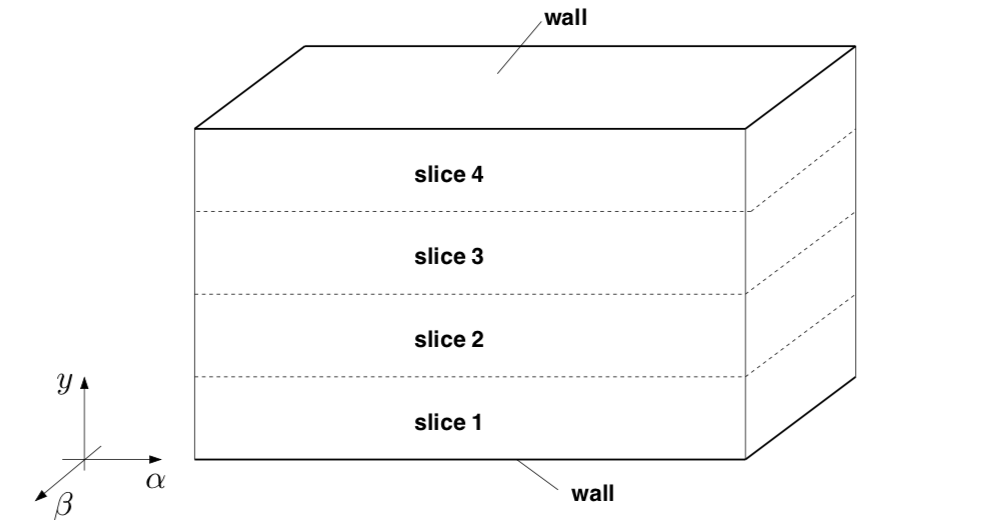
\includegraphics[width=0.5\textwidth]{grafici/decomp_dominio_cpl}
\caption{Original domain decomposition in case of 4 processors}
\label{domain_decomp}
\end{figure} allowing to perform the convolutions and relatives Fourier transformations locally on each processor, leading to a minimum of communication, moving to communication intensive decompositions, such as \emph{z-slabs}, \emph{x-slabs} or \emph{pencils}.

These solutions require communication to perform the array transpose needed by the FFTs in the two homogeneous directions